% !TEX root =  ../Dissertation.tex

\chapter{Design}

\marginpar{Add an introduction of what you want to do for each chapter}

The design of tools will describe the different systems needed to extract the
dependency graphs and analyse them. Agda Tree analyses two dependencies graphs,
one for modules and another for definitions. The module dependency graph can be
generated with Agda but for the definition dependency graph will have to be
created manually and needs to be designed.

Agda Comp is a simpler tool, as the complexity comes from testing the different
compilation strategies. It must create the module dependency graph, apply the
given strategy using the parameters provided the user and run the compilation
order. 


\pagebreak

\section{Agda Tree}

Agda Tree is a command line interface that allows the user to interact with the
module and definition graph. The first command that has to be designed is how
the CLI will create both dependency graphs. Figure \ref{fig:Agda Create Tree
Diagram} shows how the user will interact with the CLI to create the garphs.
The user provides the Agda file that they want to analyse, normally this would
be the entire project. The "Everything Index File" is the file that imports all
the modules in a project, this allows the user to analyse the entire project.
This is standard in Agda, as this is the only way to get a file that type
checks the whole project. Depending on the Agda project, this file will be
generated automatically or by the project maintainers.
\begin{figure}[H]
    \centering
    \label{fig:Agda Create Tree Diagram}
    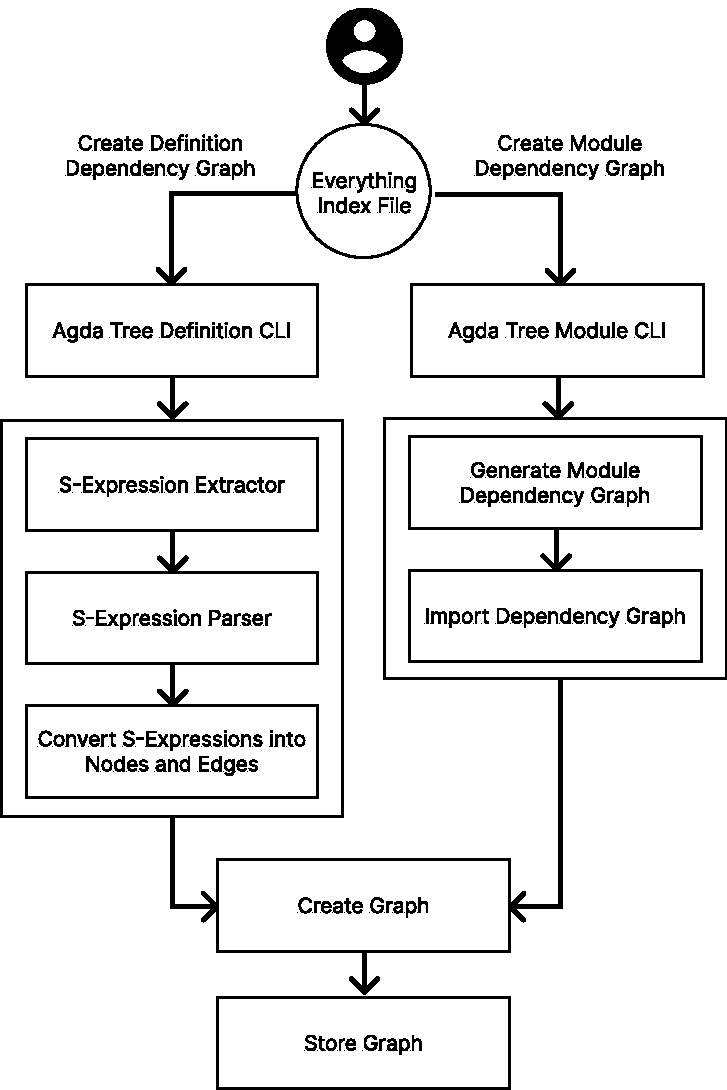
\includegraphics[scale=0.8]{Agda Create Tree.pdf}
    \caption{Agda Create Tree Diagram}
\end{figure} 

\pagebreak

Figure \ref{fig:Agda Tree Class Diagram} is a Class Diagram, showing the
classes and methods needed to operate the command line. The program starts with
the command line entry point, that will parse the input by the user and
delegate the running of the commands to the respective dependency graph. The
command line stores the default path to the dependency graph, the definition
and module dependency graph will have their own commands that can be run on
them. These queries can be found in Table \ref{table:Definition Graph Queries}
for the definition graph and in Table \ref{table:Module Graph Queries} for the
module graph for the module graph.

For the definition graph to be created, it depends on the s-expression
extractor and parser. They will read the Agda projects and convert the data
found into a graph.

\begin{figure}[H]
    \centering
    \label{fig:Agda Tree Class Diagram}
    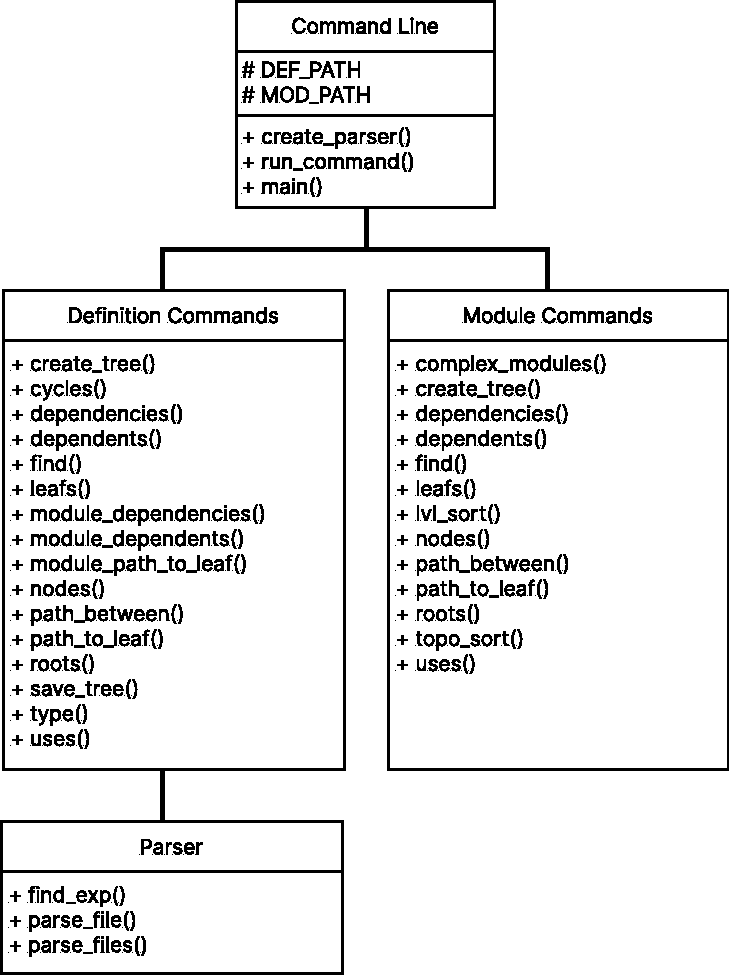
\includegraphics[scale=0.8]{Agda Tree Class Diagram.pdf}
    \caption{Agda Tree Class Diagram}
\end{figure} 
    
\pagebreak

Figure \ref{fig:Agda Tree Query Diagram} shows how the CLI splits into two,
depending on what dependency graph is being queried. When a user makes a query,
they will select the dependency graph and the respective methods will perform
that query. The output will be displayed in stdoutput, this makes sure that the
output can then be used with other commands like piping and xargs.

\begin{figure}[H]
    \centering
    \label{fig:Agda Tree Query Diagram}
    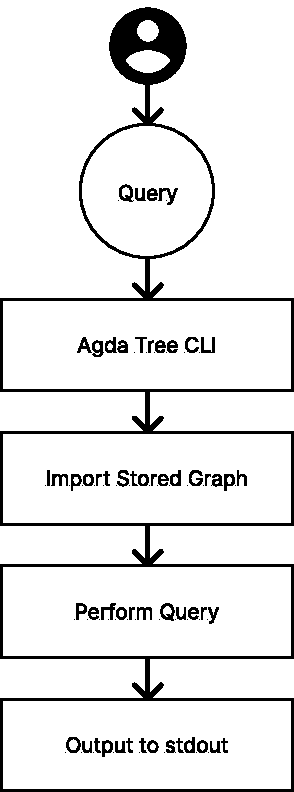
\includegraphics[scale=0.8]{Agda Make Query.pdf}
    \caption{Agda Tree Query Diagram}
\end{figure} 

\pagebreak 

\section{Agda Comp}

\marginpar{Add more stuff about Agda Comp, I don't know what}
\marginpar{What are the algorithms that are going to be sued for Agda comp}

Figure \ref{fig:Agda Comp Diagram} demonstrates how the user will interact with
the Agda Tool. The user provides the module that will be compiled, next to some
parameters defining the amount of cores used in the parallelization and what
compilation strategy to use.
\begin{figure}[H]
    \centering 
    \label{fig:Agda Comp Diagram}
    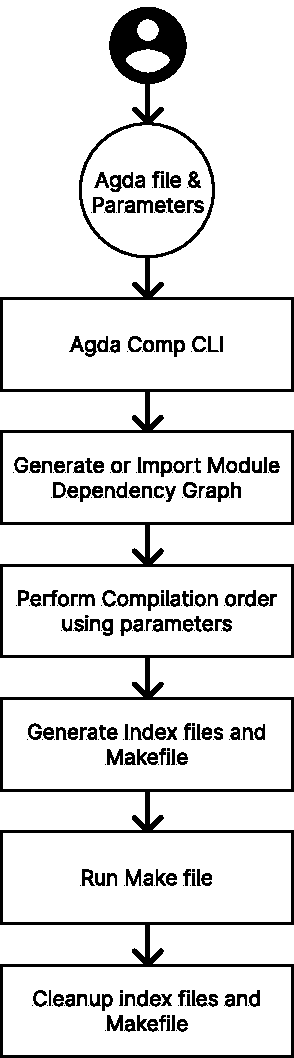
\includegraphics[scale=0.8]{Agda Comp.pdf}
    \caption{Agda Comp Diagram}
\end{figure} 


\pagebreak

\section{Conclusion}

The diagram in figure \ref{fig:Agda Tree Class Diagram} show how the structure
of the program. Figures \ref{fig:Agda Create Tree Diagram} and \ref{fig:Agda
Tree Query Diagram} also shows how the dependency graphs will be created and
how the user will interact with CLI. This structure will be important as it
ensures that the CLI can handle all the requirements and gives the project a
solid foundation to refer back to. 

The functionality of Agda Comp is modelled in Figure \ref{fig:Agda Comp
Diagram}, this structure allows the user to select what compilation strategy to
use and how many cores the compilation can use. Agda Comp is meant to allow the
user to easily apply the compilation strategies that are going to be explored
in chapter \ref{ch:implementation}.

% Communicating how you think about the composition of your system and how it
% works. You might detail the ways in which the overall system will be broken
% down into subsystems. Detail should then be provided on the design of each of
% these subsystems.
%
% \begin{itemize} \item A system that turns agda into s-expressions \item A
% system that reads s-expressions and turns it into a graph \item A system that
% queries that graph \item A way to store the graph for future use
% \end{itemize}
